% !TEX root = ../../main.tex

\chapter{Cost Estimation}

\label{chapter:cost-estimation}
In this chapter, we share the results of our experiments and explain how we used these results to build four different cost models. The \hyperref[sec:5-motivation]{first section} shows the results of the experiments, motivating why a cost model is necessary. In \autoref{sec:5-cost-models}, we talk about how we used these results to create the cost models. Each model is made for a specific purpose and offers different ways to solve the problem. This chapter aims to give a clear picture of how we ran the experiments and built the cost models from the results.

\section{Motivation}
\label{sec:5-motivation}
\todo{Simple visualisation to show why cost estimation is needed, and obvious correlations between dependent/independent vars.}
To show the major impact our chosen independent variables have on the trade-off between Materialization and Factorization we first show the performance ratio ($\frac{\text{Time}_M}{\text{Time}_F}$) against a range of independent variables.
We group the Data and Model characteristics as they both influence the actual computations being executed. The hardware characteristics influence how these computations are carried out on the hardware and are discussed separately. All figures and values in this section are computed from the experiments with synthetics datasets, unless specified otherwise.

\subsection{Data \& Model Characteristics}


\subsection{Hardware Characteristics}
The hardware used for computation impacts the runtime of a program, but here we show it also impacts the F/M trade off. Different compute unites (i.e., CPU or GPU type) have a different decision boundary for when to use Factorization over Materialization. This is shown in \autoref{fig:5-gpu-characteristics}. Differing hardware impacts the performance ratio differently per operator. For example, the (mean$\pm$std.) performance ratio of transposed Left Matrix Multiplication on the P100 is $3.03\pm2.70$, while on the V100 it is slightly lower with $2.32\pm2.21$. But, for Left (scalar) multiplication the V100 has the higher performance ratio of $0.21\pm0.04$, against the P100's lower $0.19\pm0.05$.

\begin{figure}[ht]
    \centering
    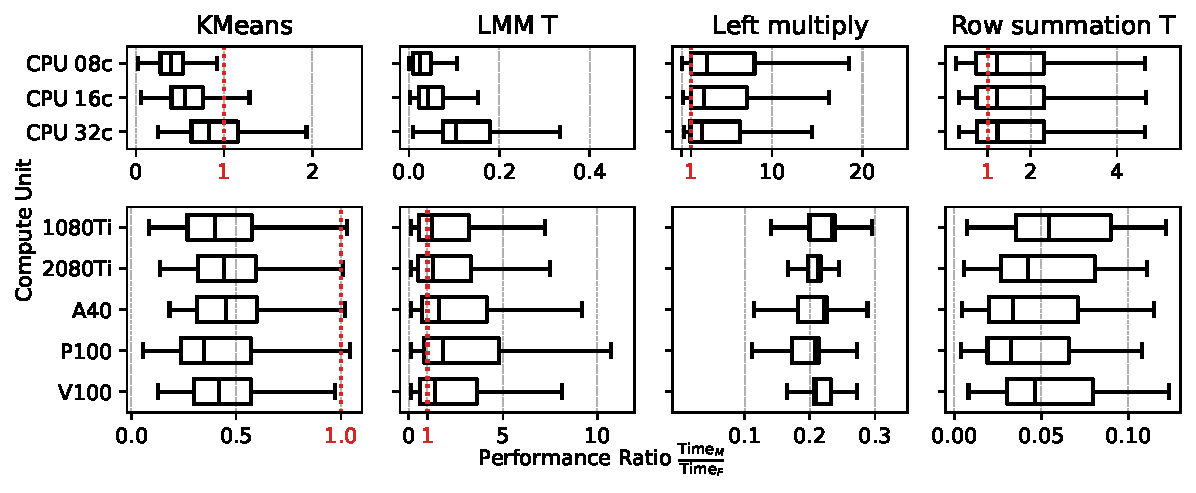
\includegraphics[width=\linewidth]{chapters/05_cost_estimation/figures/motivation_speedup_per_operator_per_gpu.pdf}
    \caption[Performance ratio plotted against hardware]{Performance ratio, of various operators on synthetic data, against hardware. The performance ratio is shown to be affected by hardware choice.}
    \label{fig:5-gpu-characteristics}
\end{figure}

\begin{table}[ht]
    \centering
    % LTeX: enabled=false
\begin{tabular}{lrrrr}
\toprule
Compute Unit & Mean & Std. Dev. & Count & \% with Speedup \\
\midrule\midrule
CPU 08c & 1.27 & 0.25 & 172 & 1.78\% \\
CPU 16c & 1.32 & 0.34 & 579 & 5.99\% \\
CPU 32c & 1.48 & 0.46 & 2873 & 29.74\% \\
1080Ti & 2.27 & 1.60 & 432 & 4.47\% \\
2080Ti & 1.87 & 1.09 & 425 & 4.40\% \\
A40 & 2.00 & 1.20 & 392 & 4.06\% \\
P100 & 2.52 & 1.84 & 461 & 4.77\% \\
V100 & 1.95 & 1.13 & 404 & 4.18\% \\
\bottomrule
\end{tabular}

    \caption[Performance ratio of ML models for cases where factorization has positive impact.]{Mean performance ratio of ML models for cases where Factorization is preferred over Materialization (speedup > 1). This shows hardware choice is a large factor in when to choose Factorization over Materialization. \todo{Make this into a plot?}}
    \label{tab:5-speedup-per-gpu}
\end{table}

If we investigate these differences between GPUs further we see that, for cases where Factorization is preferred over Materialization ($\text{Time}_F < \text{Time}_M$), there are large differences between the GPUs. Both the mean performance ratio, and the count of cases where F is faster than M varies greatly, as shown in \autoref{tab:5-speedup-per-gpu}. This shows that the choice of hardware is a large factor in when to choose Factorization over Materialization.



\section{Cost Models}
\label{sec:5-cost-models}
\todo{Detail the full process going from data to Cost model, what features where used, and what is the inner architecture?\\Show each of the factors is significant. Data, Hardware, Model parameters}

\subsection{Feature Engineering}
\label{sec:5-feature-engineering}
\todo{Data Preprocessing steps}


\subsection{Analytical}

\subsection{Statistical}

\subsection{Deep Learning}

\subsection{Hybrid}

\subsection{Meta-results}
\todo{Inference speed, training time.}
